% Created 2017-09-18 lun 14:27
\documentclass{article}
\usepackage[utf8]{inputenc}
\usepackage[T1]{fontenc}
\usepackage{fixltx2e}
\usepackage{graphicx}
\usepackage{longtable}
\usepackage{float}
\usepackage{wrapfig}
\usepackage{rotating}
\usepackage[normalem]{ulem}
\usepackage{amsmath}
\usepackage{textcomp}
\usepackage{marvosym}
\usepackage{wasysym}
\usepackage{amssymb}
\usepackage{hyperref}
\tolerance=1000
\author{Nicola Roberto Zema}
\date{\textit{<2017-09-06 mer>}}
\title{Ahmet's Robots}
\hypersetup{
  pdfkeywords={ },
  pdfsubject={},
  pdfcreator={}}
\begin{document}

\maketitle
\tableofcontents



\section{\texttt{ebug\_swarm\_control}}
\label{sec-1}

\subsection{Instructions}
\label{sec-1-1}

Just drop the \texttt{ebug\_swarm\_control} folder into
\texttt{/home/<username>/catkin\_ws/src} and issue a \verb~catkin_make~ as per
manuals/tutorials.

I have made also a launch file.

Jeez!

\subsection{Mail}
\label{sec-1-2}
Original mail from the man.
\begin{verbatim}
   Hi Nicola,
   
   Can we build a ROS structure consisting of the following blocks:

1. control_node
2. localization_node
3. planning_node
4. visualization_node
   
They will basically do nothing but exchange information through the
ROS provided (blue marked in the attached diagram) mechanisms (I
forgot the name of this whiteboard?).

If you can write a simple program in the planning_node that will
generate an initial position x,y 0 < x < 640 and 0 < y < 480 (blob
camera resolution).

control_node will read it and write it for localization_node to read.

Then the localization_node will read and write it for
visualization_node and planning_node to read.

visualization_node will have an openCV code to display a circle in a
rectangular window representing the current position of the "robot" as
a simple circle.

planning_node will read the position and generate a next position to
model a random walk of the robot. This cycle will keep going
indefinitely.

I think this will be a good starting point for us.
\end{verbatim}


\subsection{Attached Material}
\label{sec-1-3}

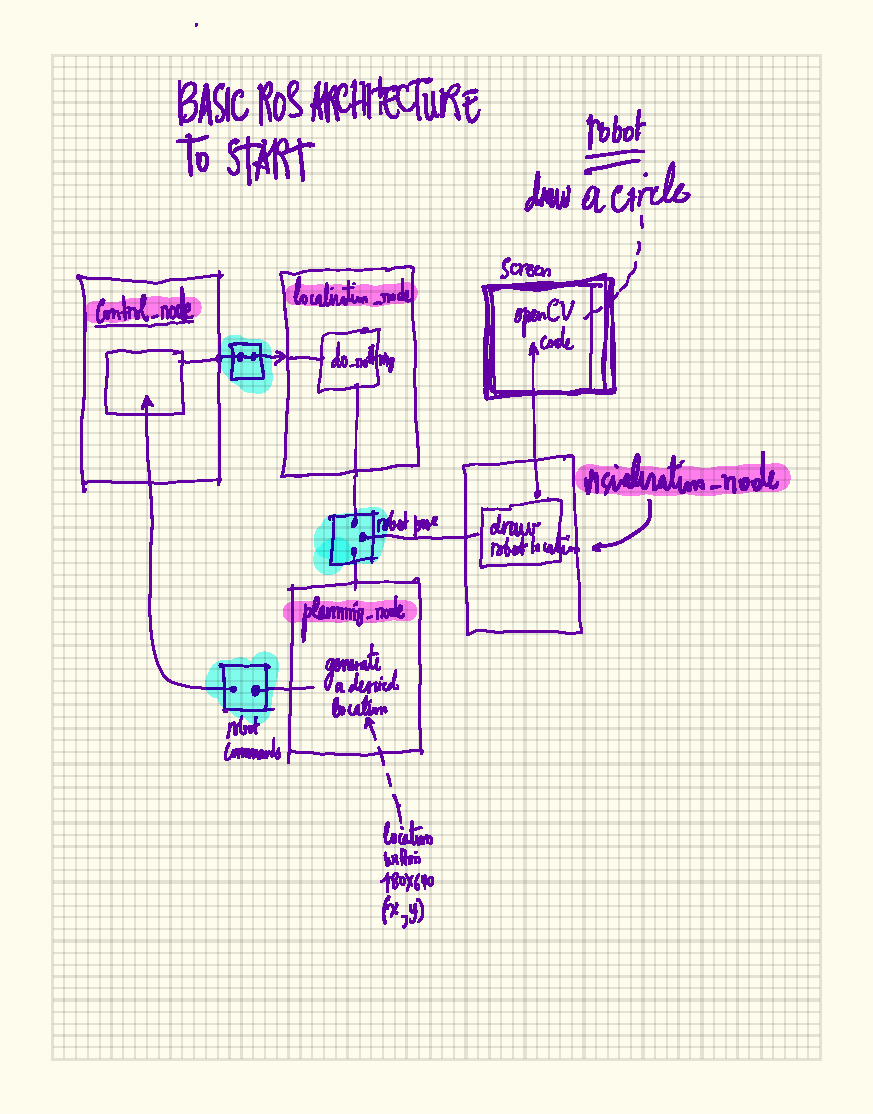
\includegraphics[width=.9\linewidth]{./material/eBugSwarm.pdf}

\subsection{Action Plan}
\label{sec-1-4}

\begin{enumerate}
\item {\bfseries\sffamily DONE} Create nodes
\label{sec-1-4-1}

\item {\bfseries\sffamily DONE} Setup makefiles and xml
\label{sec-1-4-2}

\item {\bfseries\sffamily DONE} \texttt{planning\_node}
\label{sec-1-4-3}
\begin{verbatim}
the planning_node that will
generate an initial position x,y 0 < x < 640 and 0 < y < 480 (blob
camera resolution).
\end{verbatim}
\begin{enumerate}
\item {\bfseries\sffamily DONE} basic data generation
\label{sec-1-4-3-1}
\begin{itemize}
\item It is an image \verb~640x480~;
\item It is a \texttt{sensor\_msgs/Image Message}
\item File: \texttt{sensor\_msgs/Image.msg}
\item Things to take into consideration:
\item Header header (see \ref{sec-1-4-3-1-2})
\begin{itemize}
\item WTF?!?!
\end{itemize}
\item \verb~uint32 height         # image height, that is, number of rows~
\begin{itemize}
\item Can Fake it
\end{itemize}
\item \verb~uint32 width          # image width, that is, number of columns~
\begin{itemize}
\item Can Fake it
\end{itemize}
\item \verb~string encoding       # Encoding of pixels -- channel meaning, ordering, size~
\begin{itemize}
\item Can Fake it
\end{itemize}
\item \verb~uint8 is_bigendian    # is this data bigendian?~
\begin{itemize}
\item Can Fake
\end{itemize}
\item \verb~uint32 step           # Full row length in bytes~
\begin{itemize}
\item Can Fake
\end{itemize}
\item \verb~uint8[] data          # actual matrix data, size is (step * rows)~
\begin{itemize}
\item Can Fake:
\begin{itemize}
\item Fill it with 1s
\end{itemize}
\end{itemize}
\item \textbf{ROS TAKES CARE OF ALL DEFAULTS}
\end{itemize}
\begin{enumerate}
\item How to handle it
\label{sec-1-4-3-1-1}
Send it as a message on a dedicated topic.
\item Info
\label{sec-1-4-3-1-2}
\begin{verbatim}
# This message contains an uncompressed image
# (0, 0) is at top-left corner of image
#

Header header        # Header timestamp should be acquisition time of image
                     # Header frame_id should be optical frame of camera
                     # origin of frame should be optical center of cameara
                     # +x should point to the right in the image
                     # +y should point down in the image
                     # +z should point into to plane of the image
                     # If the frame_id here and the frame_id of the CameraInfo
                     # message associated with the image conflict
                     # the behavior is undefined

uint32 height         # image height, that is, number of rows
uint32 width          # image width, that is, number of columns

# The legal values for encoding are in file src/image_encodings.cpp
# If you want to standardize a new string format, join
# ros-users@lists.sourceforge.net and send an email proposing a new encoding.

string encoding       # Encoding of pixels -- channel meaning, ordering, size
                      # taken from the list of strings in include/sensor_msgs/image_encodings.h

uint8 is_bigendian    # is this data bigendian?
uint32 step           # Full row length in bytes
uint8[] data          # actual matrix data, size is (step * rows)
\end{verbatim}
\end{enumerate}
\end{enumerate}
\item {\bfseries\sffamily DONE} \texttt{control\_node}
\label{sec-1-4-4}
\begin{verbatim}
control_node will read it and write it for localization_node to read.
\end{verbatim}
\begin{enumerate}
\item {\bfseries\sffamily DONE} Message Transport
\label{sec-1-4-4-1}
\begin{itemize}
\item Read the image from \ref{sec-1-4-3}
\item Rebroadcast it.
\end{itemize}
\end{enumerate}
\item {\bfseries\sffamily DONE} \texttt{localization\_node}
\label{sec-1-4-5}
\begin{verbatim}
the localization_node will read and write it for
visualization_node and planning_node to read.
\end{verbatim}
\begin{enumerate}
\item {\bfseries\sffamily DONE} Message Transport
\label{sec-1-4-5-1}
Same as \ref{sec-1-4-4}
\end{enumerate}
\item {\bfseries\sffamily DONE} \texttt{visualization\_node}
\label{sec-1-4-6}
\begin{verbatim}
visualization_node will have an openCV code to display a circle in a
rectangular window representing the current position of the "robot" as
a simple circle.
\end{verbatim}
\begin{enumerate}
\item {\bfseries\sffamily DONE} Data Endpoint
\label{sec-1-4-6-1}
Just print out some stuff.
\end{enumerate}
\end{enumerate}


\section{OLD}
\label{sec-2}
\subsection{Original Request}
\label{sec-2-1}

\begin{enumerate}
\item Important stuff
\label{sec-2-1-1}

\begin{enumerate}
\item Github repo
\label{sec-2-1-1-1}

\url{https://github.com/monash-wsrn/ebug2014-qt}
\end{enumerate}

\item Other mail
\label{sec-2-1-2}

Erwin has disentangled the localization routines from the of others
(He was a great student, works at the Seagate R\&D center now).

\item 
\label{sec-2-1-3}
We have an independent program that processes the blob trace and
reports the eBug positions and orientation. We have tested it with
only one stationary eBug though. I will need to collect more trace
data.
\item 
\label{sec-2-1-4}
Here is an extract from his program:
The eBug is nicely sitting at the position 665, 502 with an
orientation angle 262 degrees :-)
\item 
\label{sec-2-1-5}
I will need to check out the camera view 0,0 point and the coordinates
of other corners to determine the limits. Also will work out the
reported angle's reference angular position.
\item 
\label{sec-2-1-6}
ID =  4 x = 664.927     y = 502.462     angle = 262.533
ID =  4 x = 664.991     y = 502.46      angle = 262.393
ID =  4 x = 664.722     y = 502.149     angle = 262.707
ID =  4 x = 664.823     y = 502.443     angle = 262.484
ID =  4 x = 664.898     y = 502.411     angle = 262.479
ID =  4 x = 664.868     y = 502.622     angle = 262.447
ID =  4 x = 664.765     y = 502.315     angle = 262.713
ID =  4 x = 664.825     y = 502.456     angle = 262.642
ID =  4 x = 665.045     y = 502.419     angle = 262.406
ID =  4 x = 664.864     y = 502.598     angle = 262.393
ID =  4 x = 664.943     y = 502.307     angle = 262.572
\item 
\label{sec-2-1-7}
So \ldots{} I think eBug localization with RGB LED tracking is under
control. If you can, I will need your continuing help on trajectory
control block.
\end{enumerate}

\subsection{New Robots}
\label{sec-2-2}

\begin{enumerate}
\item Mail 1
\label{sec-2-2-1}
Hi Nicola,

I attach my thinking about the  ROS based architecture of the eBug
Swarm Control System (running on Linux). There are three independent
processes (in ROS parlance, "nodes", I think).
\item 
\label{sec-2-2-2}
Big rectangle at the left is the only one that has connection with the
radio, and gets camera blobs, sends eBug control commands. This one is
pretty much under control.
\item 
\label{sec-2-2-3}
Small rectangle at the upper right corner is the one that we attempted
to extract from Erwin's code. I'm trying to contact Erwin to see
whether I can get him to do it.
\item 
\label{sec-2-2-4}
Small rectangle at the lower right is the place perhaps you can help.
What I want at the moment is a small demo, say 5 eBugs that to do
something interesting. Simplest possibility I can think of is to
pre-calculate trajectories for each eBug in a way that they won't
collide and send periodical commands to maintain the desired
trajectories. Do you think you can help with this?
\item 
\label{sec-2-2-5}
A more challenging approach would be to extract control modules from
Erwin's code and reuse withing the ROS context I have drawn.
\item 
\label{sec-2-2-6}
Please let me know what you think.
\item Material
\label{sec-2-2-7}
\texttt{material/scan\_asekerci\_2017-09-04-16-07-11.pdf}

\item Python files
\label{sec-2-2-8}

\begin{enumerate}
\item nrf.py library and a short sample python code
\label{sec-2-2-8-1}

\url{./nrf.py}

\url{./discover.py}
\end{enumerate}
\end{enumerate}
\end{document}